\chapter{\IfLanguageName{dutch}{Stand van zaken}{State of the art}}
\label{ch:stand-van-zaken}

% Tip: Begin elk hoofdstuk met een paragraaf inleiding die beschrijft hoe
% dit hoofdstuk past binnen het geheel van de bachelorproef. Geef in het
% bijzonder aan wat de link is met het vorige en volgende hoofdstuk.

% Pas na deze inleidende paragraaf komt de eerste sectiehoofding.


In dit deel zal men toespitsen op de werking van een wayfinding applicatie, bij uitstek de concrete werking van het AI/AR mechanisme.

\section{AI (Artificiële intelligentie)}
Artificiële intelligentie of AI is een zeer groot fenomeen in de huidige IT-wereld. Men kan het beschrijven als intelligentie die wordt gedemonstreerd door machines. Op deze manier kunnen die apparaten de omgeving waarnemen en vervolgens acties ondernemen die het succesvol bereiken van een bepaald doel zal maximaliseren. In het algemeen staat de term AI ook gekend als de beschrijving van machines of computers die cognitieve acties uitvoeren die wij als mensen associeren met de menselijke geest. 

In deze bachelorproef wordt AI toegepast op het vlak van objectdetectie, het is de meest cruciale factor om een wayfinding applicatie te optimaliseren.
Objectdetectie zal in de wayfinding applicatie er voor zorgen dat de omgeving op een correcte manier wordt herkend, zo kan men een perfect beeld scheppen van welke objecten men afstand moet houden, bijvoorbeeld muren.

\subsection{Objectherkenning vs. Objectdetectie}
In Artificiële intelligentie heeft men twee verschillende manieren om objecten te identificeren, objectherkenning en objectdetectie. Het herkenningsproces is zeer gelijkaardig, maar toch zijn er zekere verschillen bij de uitvoering. Objectdetectie kan men beschouwen als een subset van objectherkenning, men zal de objecten herkennen op een simultane manier, maar bij objectdetectie wordt het object ook gelocaliseerd in de afbeelding. In de onderstaande afbeelding kan men het verschil duidelijk waarnemen, objectherkenning (links) en objectdetectie (rechts).

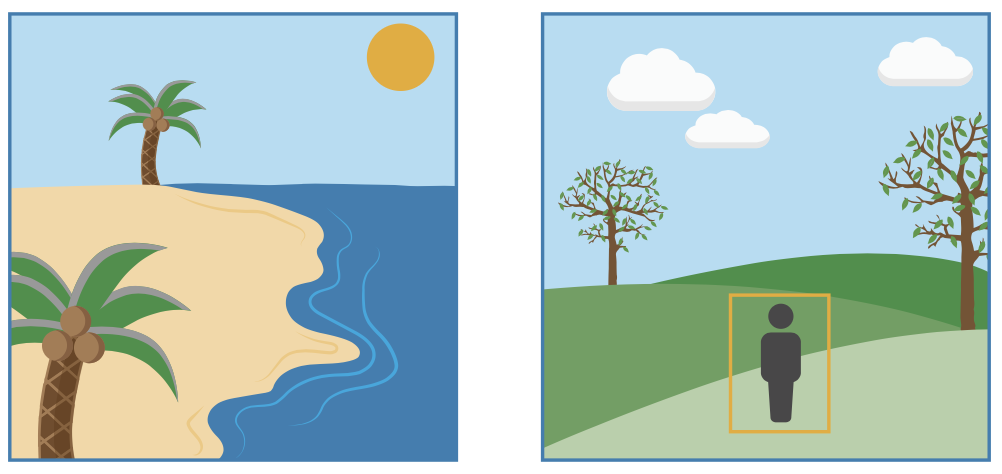
\includegraphics[scale=0.5]{objectdetectie.png}

\subsection{Werking van objectherkenning}
Om objectherkenning toe te passen kan je gebruik maken van twee verschillende manieren, namelijk 'Machine Learning' en 'Deep learning'. Beide technieken zullen objecten gaan herkennen, maar ze zijn verschillend op vlak van uitvoering.

\subsubsection{Machine learing}
Machine learning maakt gebruik van classificatie om een bepaald object te herkennen. Ten eerste zal men een trainingset opstellen, dit gebeurt door een verzameling van afbeeldingen samen te stellen en vervolgens de relevante punten aan te duiden. Het is zeer belangrijk om de juiste relevante punten aan te duiden, anders zal het systeem verkeerd getraind worden, waardoor men vervolgens een verkeerde output zal verkrijgen. Deze punten zullen er voor zorgen dat het systeem verschillende categorieën herkent. Vervolgens zal het leermodel deze informatie gebruiken om nieuwe objecten (objecten die nog niet gekend zijn in de trainingset) te analyseren en te classificeren.

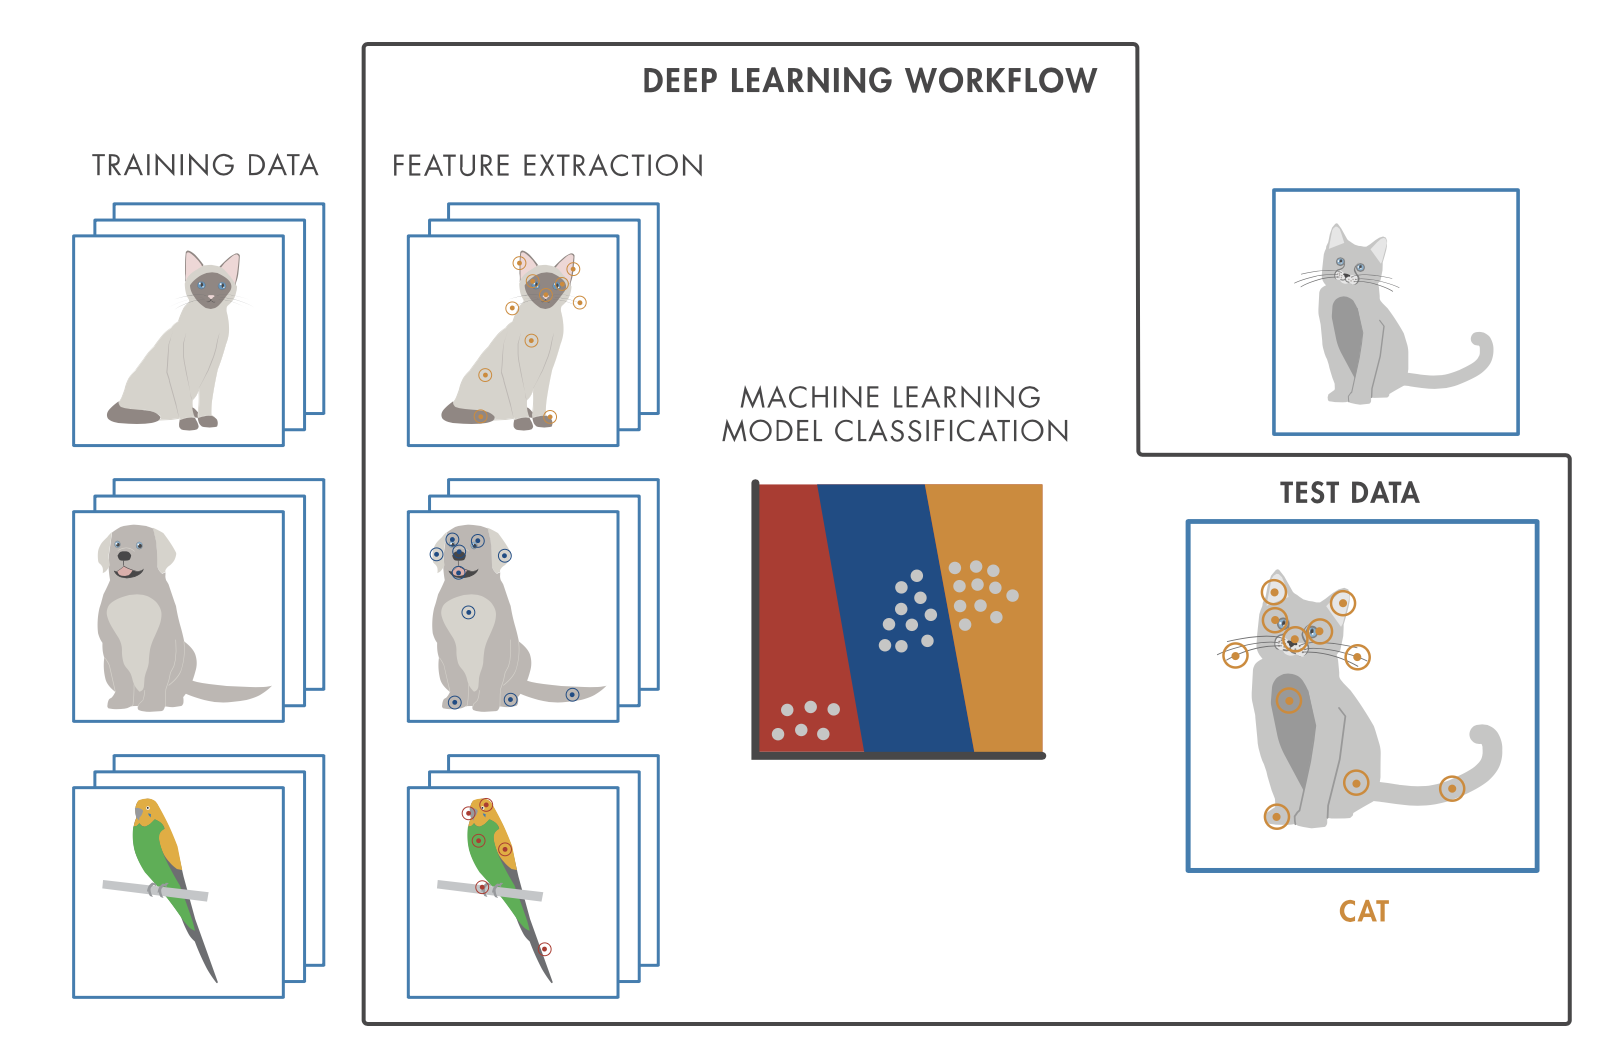
\includegraphics[scale=0.4]{machinelearning.png}

\subsubsection{Deep learning}
Deep learning maakt gebruik van convulationele neurale netwerken (CNN) om objecten te herkennen. Een CNN kan automatisch de aanhangende kenmerken van een object leren om dat object te identificeren, dit betekent dat een CNN bijvoorbeeld het verschil tussen auto's en vrachtwagens kan herkennen door middel van duizenden afbeeldingen te analyseren en vervolgens te leren welke kenmerken juist verschillend zijn.

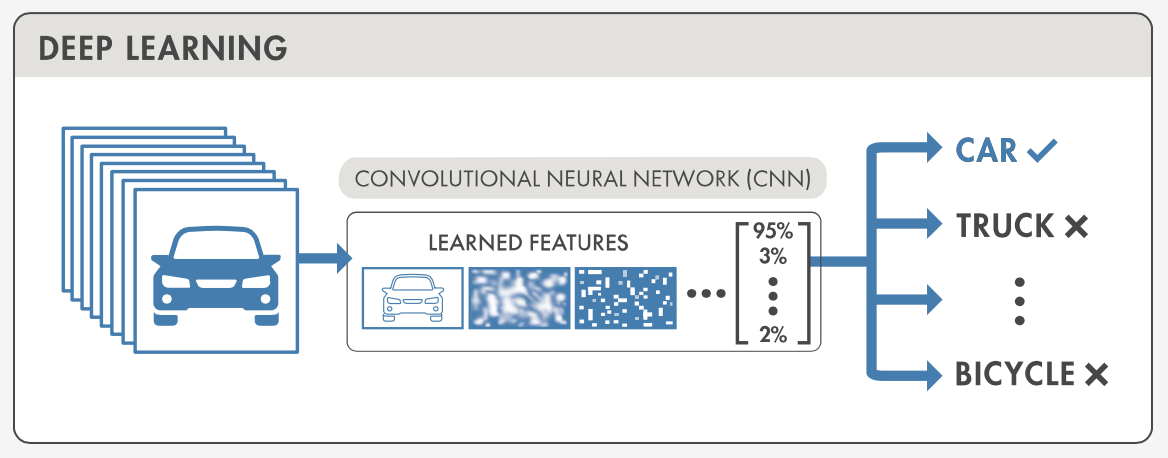
\includegraphics[scale=0.6]{deeplearning.png}
\section{AR (Augmented reality)}
Augmented reality (AR) is een interactieve ervaring van de echte wereld waarin objecten die zich in de echte wereld bevinden worden versterkt door computergegenereerde objecten, in een wayfinding applicatie gebeurt dit door middel van pijlen die de route aangeven.

Het doel van Augemented reality in deze bachelorproef is om de route op een zo efficiënt mogelijke manier aan te geven, dit betekent dat er geen pijlen door objecten mogen gaan.

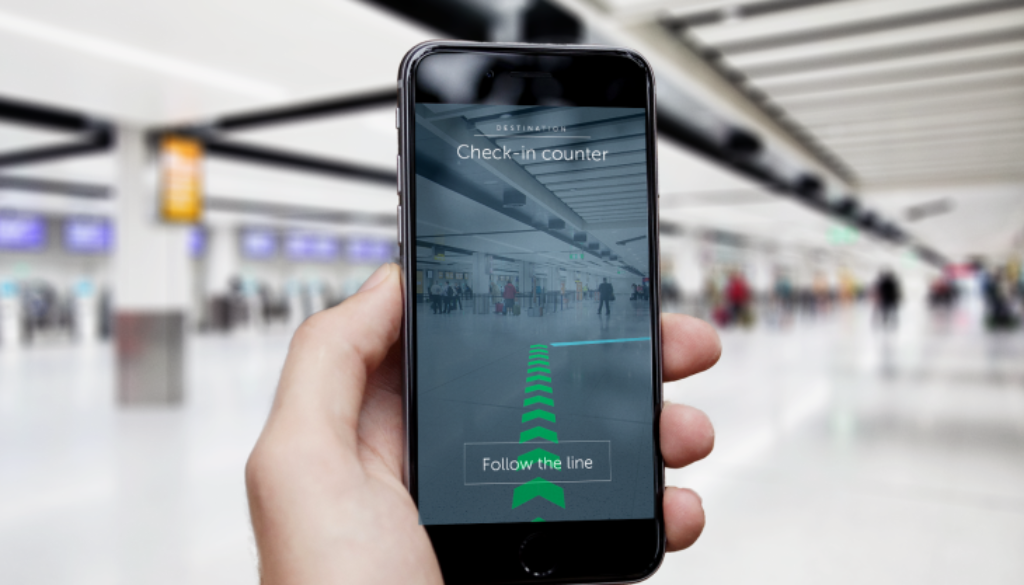
\includegraphics[scale=0.3]{wayfinding.png}
\section{AI + AR}
De samenhang van Artificiële intelligentie en Augmented reality is zeer cruciaal bij het optimaliseren van een wayfinding applicatie. Ten eerste is het belangrijk dat de objecten op een correcte manier worden herkend. Ten tweede is het zeer belangrijk dat de bevindingen van de objectherkenning op een correcte manier worden vertaald naar de AR omgeving. Dit stuk is het meeste cruciale punt van deze bachelorproef.


